\documentclass[authoryear, 12pt,5p, times]{elsarticle}
%\usepackage[hypcap]{caption}
%\geometry{margin=0.95in,top=1.4in,bottom=1.4in}
\geometry{margin=1in,top=1.3in,bottom=1.3in}
\usepackage{float}
\usepackage{amsmath}
\usepackage[hidelinks]{hyperref} 
 \usepackage{gensymb}
\usepackage{subcaption}
\usepackage{url}
%\renewcommand\thefootnote{\fnsymbol{\dagger}}
\usepackage[symbol*]{footmisc}
\newcommand{\rpm}{\raisebox{.2ex}{$\scriptstyle\pm$}}
\begin{document}
%\footnote{This is a footnote}
\begin{frontmatter}
\title{Asteroid Astrometry from CCD Images}
\author{\today \\ \quad \\Jung Lin (Doris) Lee\\ dorislee@berkeley.edu\\Group partners: Jennifer Ito, Manuel Silvia\\Prof. James Graham, UGSI Heechan Yuk, Isaac Domagalski}
	\begin{abstract}
In this experiment,  we------
we use the method of least squares to calibrate the wavelength calibration 
	\end{abstract}
\end{frontmatter}
\section{Introduction}
\section{Data Reduction}
\subsection{Dark, Bias, Flat Subtraction}
\label{subtraction}
Using the halogen lamp as a source of uniform illumination, the flat field images calibrate the pixel-by-pixel variations as well as common artifacts that is seen in both continuum sources as shown in Fig. \ref{calib}. We take the ``dark frame" as the the average of the ---- (i.e. the flat region shown in Fig. ----) before and after the  . Without subtracting the bias in the ``dark image", we can automatically get bias subtraction by simply subtraction off the dark, as the bias is incorporated as part of the ``dark frame" .
Every image pixel is:
\begin{equation}
			\frac{\text{image}-\text{dark}}{\text{flat}}\times\text{median(flat)}
			\label{calib_eq}
\end{equation}
 \begin{figure}[h!]
 When converting the 2D images to 1D spectra, we took a 1024-by-1024 pixel slice of the image array to truncate the 24 overscan pixels.
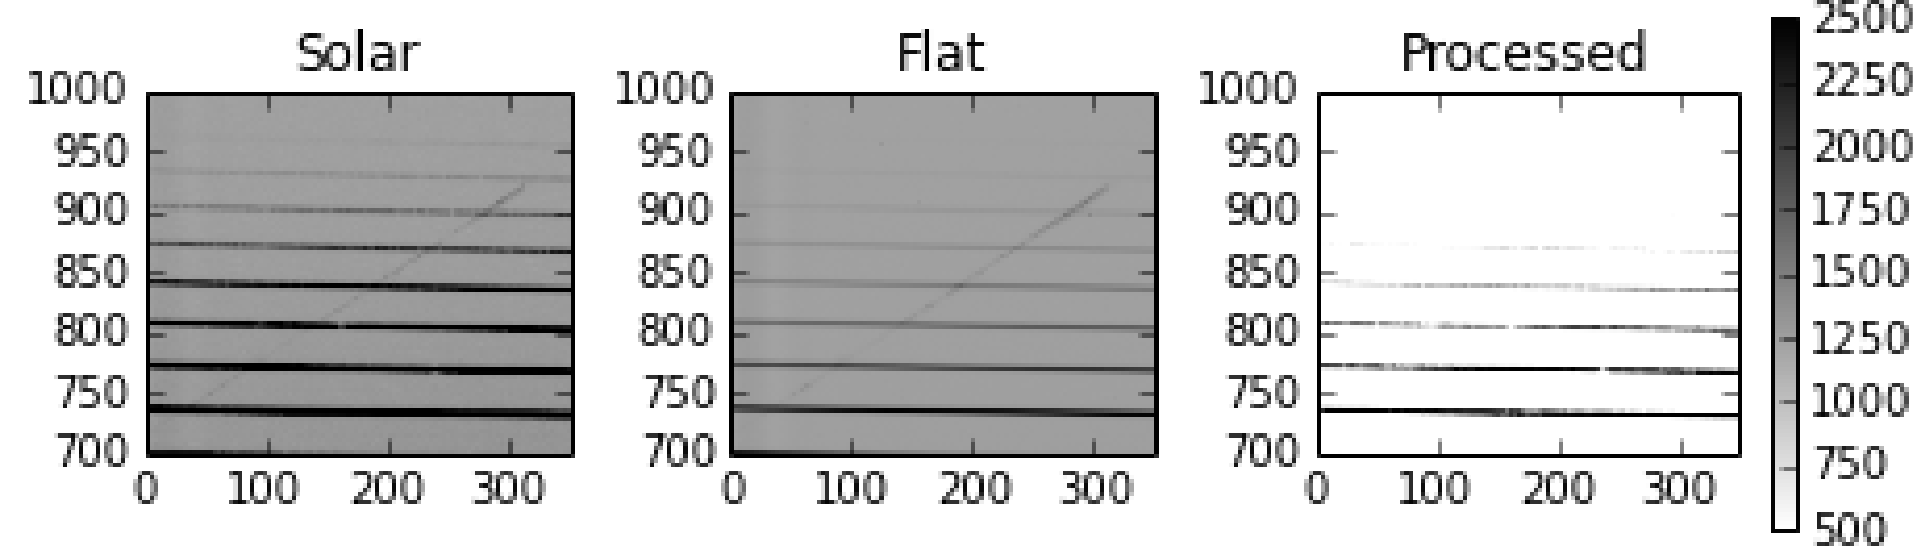
\includegraphics[width=0.5\textwidth]{figures/processed}
\caption{Both continuous sources shows the same artifact in a corner of the CCD image. The figures below are zoomed in --- on this feature, which  possibly from the reflected light . The halogen exposure is used for flat correction. Along with subtracting the background from the non-incident solar spectrum, the artifact is removed in the proceessed image shown in the rightmost figure.}
\label{processed}
\end{figure}
\subsection{Spectrometer details}
The table below shows ---- for m=35 
Echelle order of interference on blaze (m)

\subsection{Wavelength Calibration}
From the halogen spectrum we deduced that the cross-dispersion wavelength ( $\lambda_{cd}$)decreases along the direction of y axis and from the tilted order, we conclude that the wavelength from the echelle grating ($\lambda_{e}$) increase from right to left.
We took exposures where both the neon light and 635nm green laser was turned on in order to identify  where ----- .Since each order has a slightly different coefficient, we chose to calibrate the order containing the 635nm green laser. as a convient 
\begin{figure}[h!]
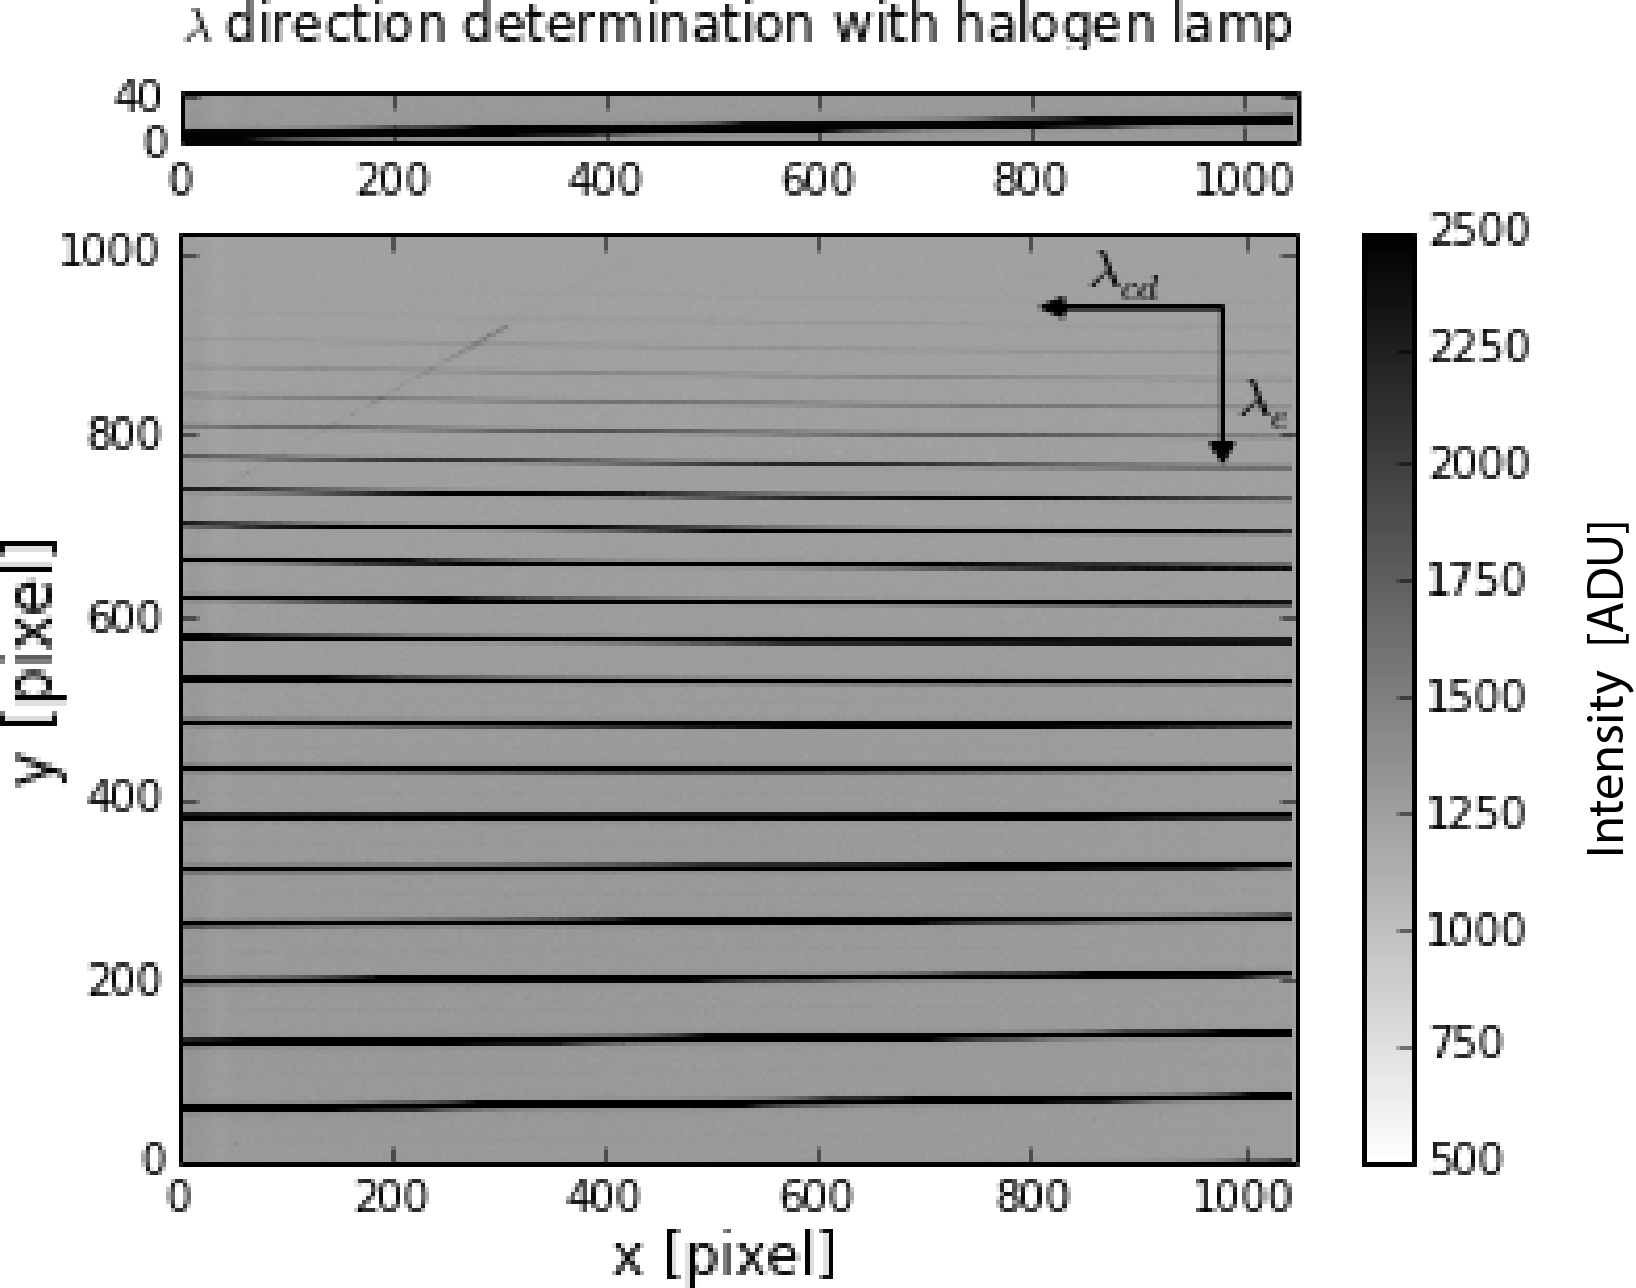
\includegraphics[width=0.5\textwidth]{figures/lambda_direction}
\caption{Wavelength direction, the arrow points in the direction of increasing wavelength. We determine the tilting direction from a zoomed-in section of a single echelle  order, as shown in the top figure.}
\label{lambda_direction}
\end{figure}
 \begin{figure}[h!]
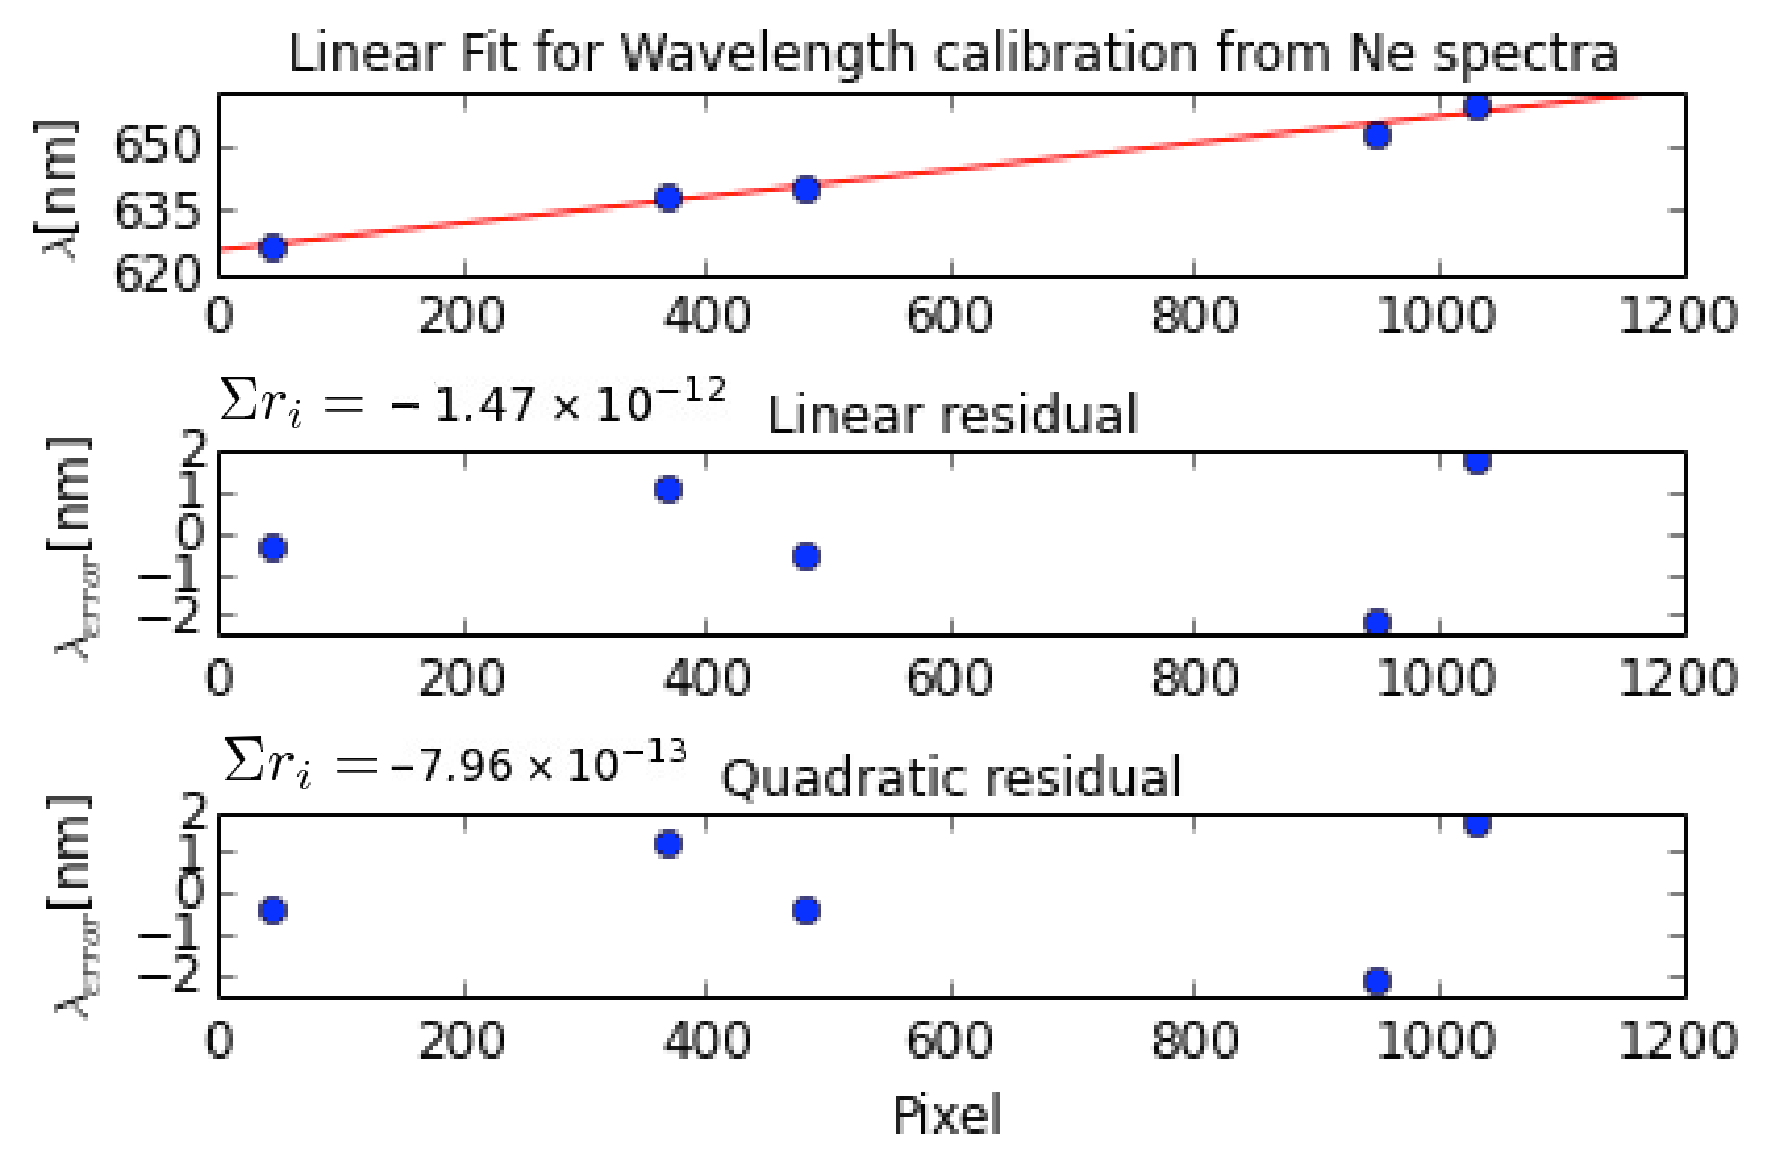
\includegraphics[width=0.5\textwidth]{figures/wavelength_calib}
\caption{The first order fit in the top figure shows that the dispersion is approximately linear ($\frac{d\lambda}{d\text{pixel}}$=0.0315 nm/pixel ). Since there is no notable patterns in linear residual and the magnitude of the residual is small, a linear relationship should be sufficient for pixel-to-wavelength conversion. From the bottom most quadratic figure, we see that the residual decrease by an order of magnitude.}
\label{calib}
\end{figure}
\section{Limb Darkening}
The data quality of the solar scan can be verified by the a time series plot as shown in Fig. \ref{eddington_fit}. Intensity fluctuation that deviates from the predicted effect of limb darkening indicates possible shading effect from presence of cloud or objects near the telescope such as a crossing observer. Qualitatively, this information can be used to visually reject entire shaded scans or pick out exposures in the bright central region for a more accurate Doppler shift determination. Quantitatively, we can also make use of the limb darkening effect to determine crossing time of the solar scan, used in our solar angular size calculation in Sec.\ref{size_calc}.
\\
\begin{figure}[h!]
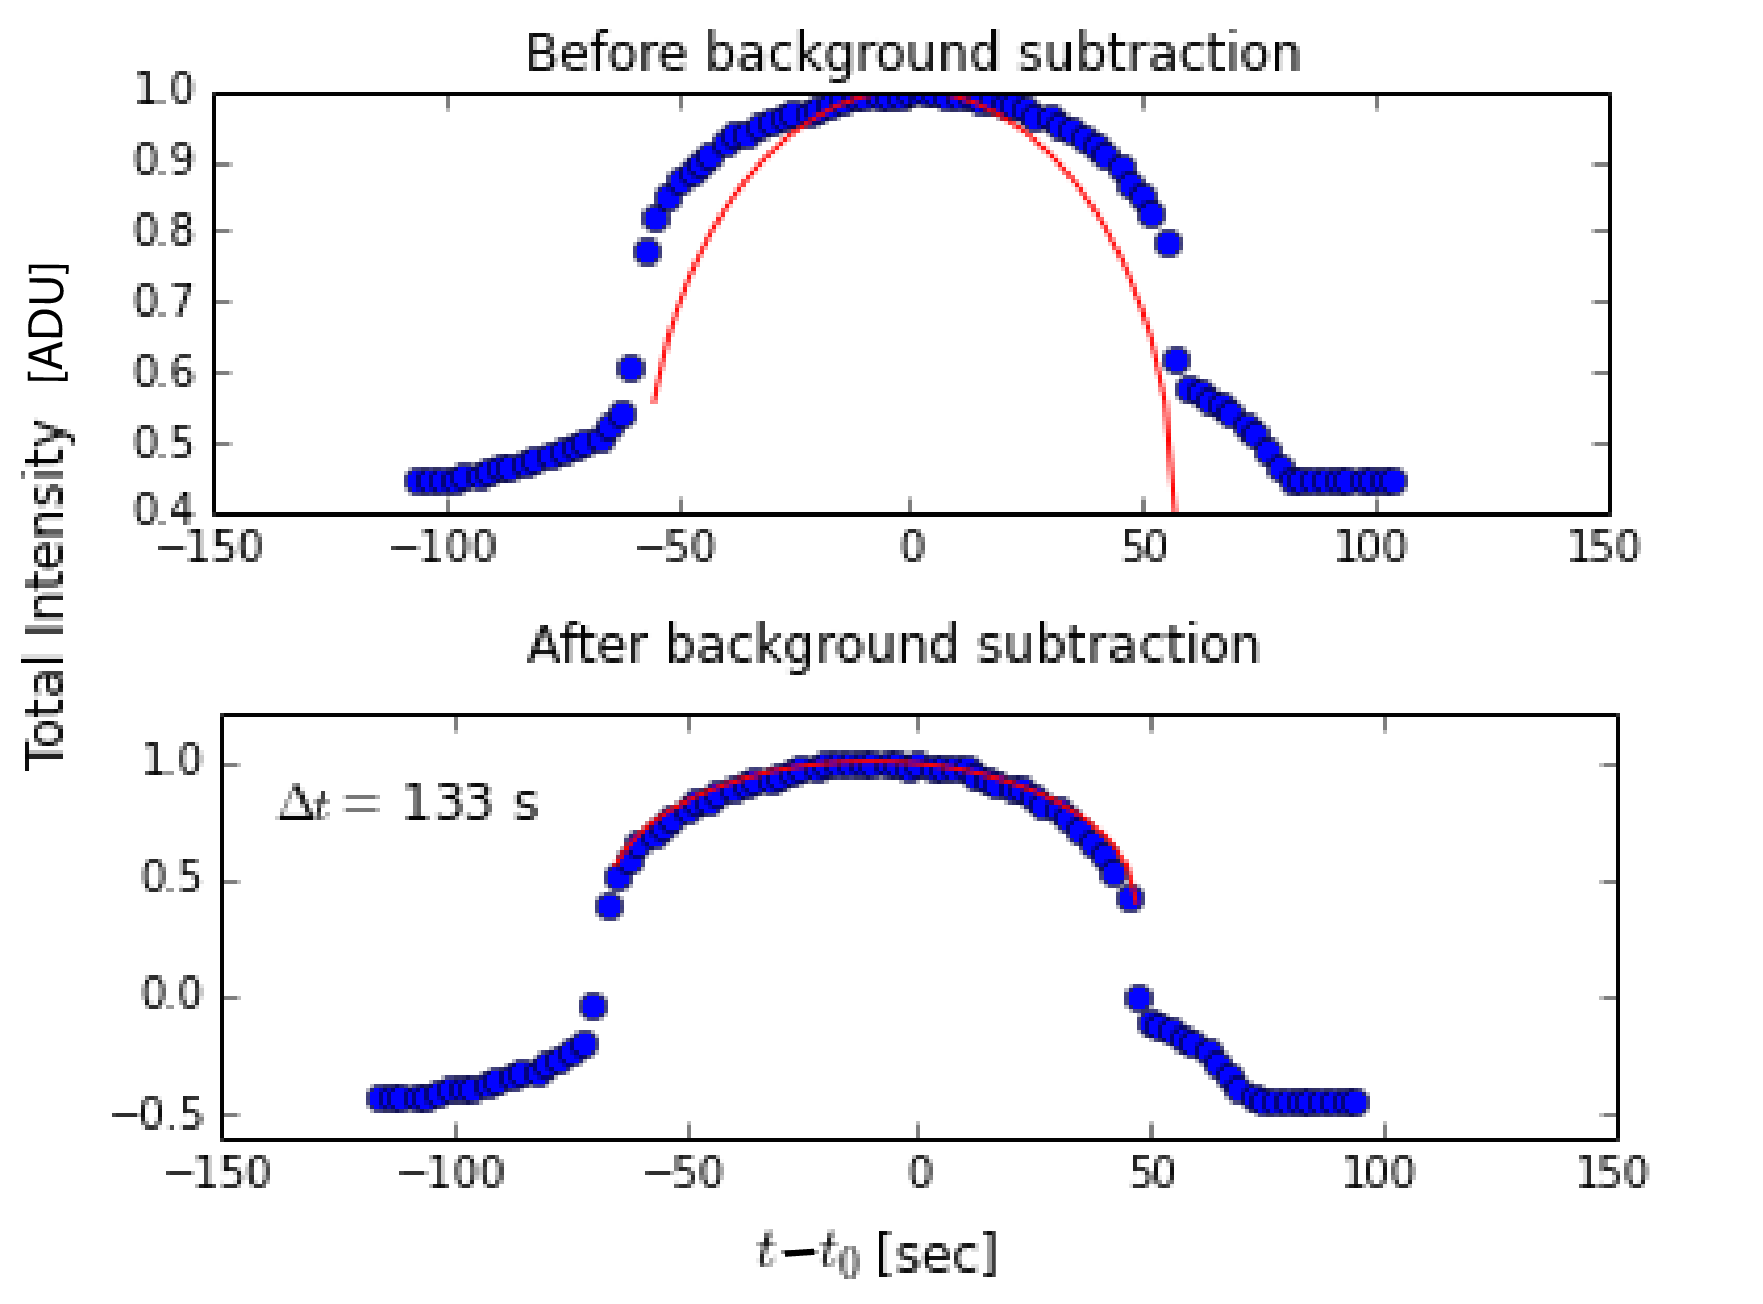
\includegraphics[width=0.5\textwidth]{figures/eddington_fit}
\caption{ The time series 
$t_0$ is the intensity of the central bright peak
The y-axis is normalized so that curve fitting corresponds to the model's output I/$I_0$ . The clear improvement of the model fit after background subtraction is evident as some of the intensity fluctuation may be mitigated by systematic effects corrected in the dark and flat frames discussed in Sec.\ref{subtraction}. }
\label{eddington_fit}
\end{figure}
\\
To avoid the arbitrary determination of the exposure that defines the start and end of the solar crossing, we fit our data to Eq.\ref{eddington_eq} with the center-to-limb time ($\Delta t$) as our varying parameter.  The lower figure in Fig.\ref{eddington_fit} shows the result of substituting the value of $\Delta t$ back into Eq.\ref{eddington_eq}, and ignoring the uneven data points on the two sides  (an artifact of the telescope) and the region before and after the solar crossing. Without this procedure, the fit would be largely distorted by the telescope artifact on the two sides and the ``dark" regions, which is not part of the stellar model. 
\\
We see the effect of limb darkening by summing together the intensity of all pixel in every CCD image in a full solar scan. Limb darkening results from the limitation that an observer can only see into a constant optical depth of 2/3. As the density and temperature of a star decreases radially outwards, the observer sees light originating from different regions of the star corresponding to the darkening effect. The time series data in Fig. --- shows the total intensity of each exposure scaled by the intensity at the central bright peak ($I_0$) which we set at the origin. By modelling intensity as a function of the incident viewing angle using the Eddington approximation for grey, plane-parallel stellar atmosphere and geometrically relating this with the Earth-sun distance and crossing times, we obtain the relation: 
\begin{equation}
\frac{I(\theta)}{I(\theta=0)}=\frac{I}{I_0}= \frac{2}{5}+\frac{3}{5}cos\theta
\label{eddington_eq}
\end{equation}
where 
By using trignometric relation 
The relative 
\section{Doppler Shift Determination}
\subsection{Cross Correlation}
\subsection{Angular Size Determination}
\label{size_calc}
\section{Conclusion}
 
 \section*{References}
 \begin{footnotesize}
 \begin{itemize}
 \item Carroll, Bradley W., and Dale A. Ostlie. \textit{An Introduction to Modern Astrophysics}. San Francisco: Pearson Addison-Wesley, 2007. Print.
\item Chromey, Frederick R. \textit{To Measure the Sky: An Introduction to Observational Astronomy}. Cambridge: Cambridge UP, 2010. Print.
\item Press, William H., and William T. Vetterling. \textit{Numerical Recipes in C: The Art of Scientific Computing}. Cambridge University Press, 1992.  
\end{itemize}
% \bibliography{references}
%\bibliographystyle{elsarticle-harv}
  \end{footnotesize}

\end{document}
